\documentclass[10pt]{article}
\usepackage[utf8]{inputenc}
\usepackage{parskip}
\usepackage[margin = 1in]{geometry}
\usepackage{xcolor}
\usepackage[colorlinks = true,linkcolor = blue, urlcolor  = blue,citecolor = blue,anchorcolor = blue]{hyperref}
\usepackage{framed}
\usepackage{apacite}
\usepackage[authoryear,sort]{natbib}
\usepackage{amsmath}
\usepackage{amssymb}
\bibliographystyle{apalike}
\newcommand{\E}{\textrm{E}}
\renewcommand{\P}{\text{P}}
\usepackage{tikz}
\usetikzlibrary{arrows,shapes.arrows,positioning,shapes,patterns,calc}

\begin{document}

\begin{Large} 
Info 6751. Fall 2022. Principal Stratification Exercise \textbf{Solutions}
\end{Large}
\hline \vskip .1in

Education promotes financial well-being and the ability to pass on opportunities to one's children. Meanwhile, college also takes time and may reduce the probability of having children at all.

\begin{center}
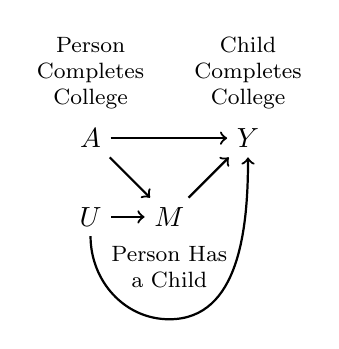
\begin{tikzpicture}
\node (a) at (0,0) {$A$};
\node (m) at (1,-1) {$M$};
\node (u) at (0,-1) {$U$};
\node (y) at (2,0) {$Y$};
\node[anchor = south, align = center, font = \footnotesize] at (a.north) {Person\\Completes\\College};
\node[anchor = north, align = center, font = \footnotesize] at (m.south) {Person Has\\a Child};
\node[anchor = south, align = center, font = \footnotesize] at (y.north) {Child\\Completes\\College};
\draw[->, thick] (a) -- (m);
\draw[->, thick] (m) -- (y);
\draw[->, thick] (a) -- (y);
\draw[->, thick] (u) -- (m);
\draw[->, thick] (u) to[out = 270, in = 180] (1,-2.3) to[out = 0, in = 270] (y);
\end{tikzpicture}
\end{center}

This creates an interesting causal structure: $Y$ is meaningless if $M = 0$.

To focus on that problem, we will assume throughout that $A$ is unconfounded: pretend that college is randomly assigned. Having a child $M$, however, may be confounded.

To solve this conundrum, suppose the population is comprised of four principal strata, which are not observed.

\begin{itemize}
\item $S = 1$: Those who would have a child regardless of whether they finished college
\item $S = 2$: Those who would not have a child regardless of whether they finished college
\item $S = 3$: Those who would have a child if and only if they did not complete college
\item $S = 4$: Those who would have a child if and only if they completed college
\end{itemize}

These strata are population subgroups that exist before treatment is assigned.

\textbf{Question 1.} What is the causal effect of college on fertility in each of the four strata?

\textbf{Answer.}
\begin{enumerate}
\item College has no effect on fertility---child in any case
\item College has no effect on fertility---no child in any case
\item College prevents having a child (-1)
\item College causes having a child (+1)
\end{enumerate} %\vskip .2in

Note that within strata 1 and 4, $M$ is not post-treatment because it is not caused by $A$. If we could restrict to these strata, we could condition on $M$ without inducing collider bias. This is why principal stratificaton is a helpful idea: it reconceptualizes a post-treatment problem into pre-treatment groups.

\begin{center}
\scalebox{.85}{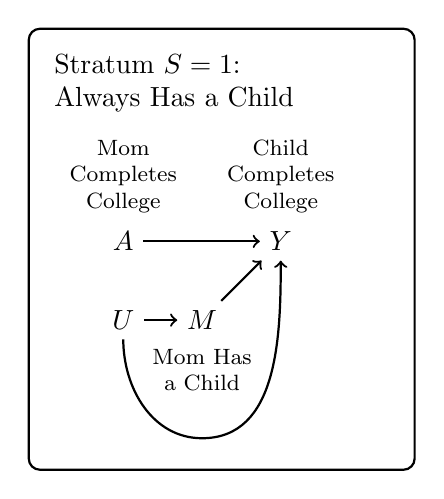
\begin{tikzpicture}
\draw[thick, rounded corners] (-1.2,2.7) rectangle (3.7,-2.9);
\node[anchor = north west, align = left] at (-1,2.5) {Stratum $S = 1$:\\Always Has a Child};
\node (a) at (0,0) {$A$};
\node (m) at (1,-1) {$M$};
\node (u) at (0,-1) {$U$};
\node (y) at (2,0) {$Y$};
\node[anchor = south, align = center, font = \footnotesize] at (a.north) {Mom\\Completes\\College};
\node[anchor = north, align = center, font = \footnotesize] at (m.south) {Mom Has\\a Child};
\node[anchor = south, align = center, font = \footnotesize] at (y.north) {Child\\Completes\\College};
\draw[->, thick] (m) -- (y);
\draw[->, thick] (a) -- (y);
\draw[->, thick] (u) -- (m);
\draw[->, thick] (u) to[out = 270, in = 180] (1,-2.5) to[out = 0, in = 270] (y);
\end{tikzpicture}
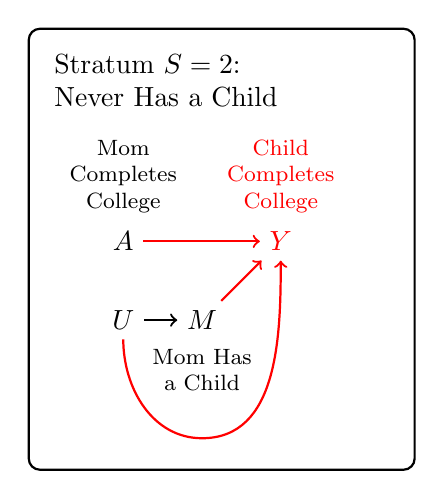
\begin{tikzpicture}
\draw[thick, rounded corners] (-1.2,2.7) rectangle (3.7,-2.9);
\node[anchor = north west, align = left] at (-1,2.5) {Stratum $S = 2$:\\Never Has a Child};
\node (a) at (0,0) {$A$};
\node (m) at (1,-1) {$M$};
\node (u) at (0,-1) {$U$};
\node[red] (y) at (2,0) {$Y$};
\node[anchor = south, align = center, font = \footnotesize] at (a.north) {Mom\\Completes\\College};
\node[anchor = north, align = center, font = \footnotesize] at (m.south) {Mom Has\\a Child};
\node[anchor = south, align = center, font = \footnotesize, red] at (y.north) {Child\\Completes\\College};
\draw[->, thick, red] (m) -- (y);
\draw[->, thick, red] (a) -- (y);
\draw[->, thick] (u) -- (m);
\draw[->, thick, red] (u) to[out = 270, in = 180] (1,-2.5) to[out = 0, in = 270] (y);
\end{tikzpicture} 
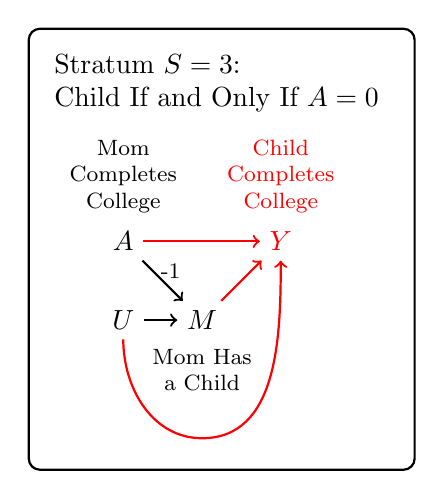
\begin{tikzpicture}
\draw[thick, rounded corners] (-1.2,2.7) rectangle (3.7,-2.9);
\node[anchor = north west, align = left] at (-1,2.5) {Stratum $S = 3$:\\Child If and Only If $A = 0$};
\node (a) at (0,0) {$A$};
\node (m) at (1,-1) {$M$};
\node (u) at (0,-1) {$U$};
\node[red] (y) at (2,0) {$Y$};
\node[anchor = south, align = center, font = \footnotesize] at (a.north) {Mom\\Completes\\College};
\node[anchor = north, align = center, font = \footnotesize] at (m.south) {Mom Has\\a Child};
\node[anchor = south, align = center, font = \footnotesize, red] at (y.north) {Child\\Completes\\College};
\draw[->, thick] (a) -- node[pos = .7, above, font = \footnotesize] {-1} (m);
\draw[->, thick, red] (m) -- (y);
\draw[->, thick, red] (a) -- (y);
\draw[->, thick] (u) -- (m);
\draw[->, thick, red] (u) to[out = 270, in = 180] (1,-2.5) to[out = 0, in = 270] (y);
\end{tikzpicture}
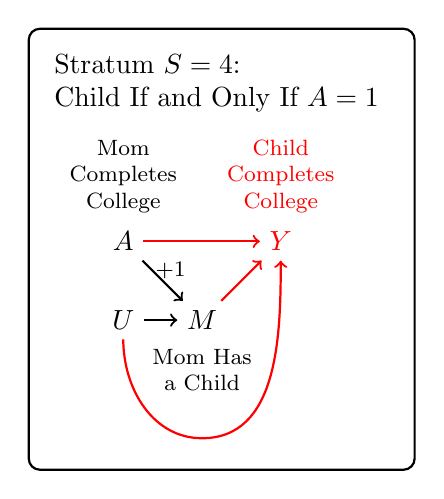
\begin{tikzpicture}
\draw[thick, rounded corners] (-1.2,2.7) rectangle (3.7,-2.9);
\node[anchor = north west, align = left] at (-1,2.5) {Stratum $S = 4$:\\Child If and Only If $A = 1$};
\node (a) at (0,0) {$A$};
\node (m) at (1,-1) {$M$};
\node (u) at (0,-1) {$U$};
\node[red] (y) at (2,0) {$Y$};
\node[anchor = south, align = center, font = \footnotesize] at (a.north) {Mom\\Completes\\College};
\node[anchor = north, align = center, font = \footnotesize] at (m.south) {Mom Has\\a Child};
\node[anchor = south, align = center, font = \footnotesize, red] at (y.north) {Child\\Completes\\College};
\draw[->, thick] (a) -- node[pos = .7, above, font = \footnotesize] {+1} (m);
\draw[->, thick, red] (m) -- (y);
\draw[->, thick, red] (a) -- (y);
\draw[->, thick] (u) -- (m);
\draw[->, thick, red] (u) to[out = 270, in = 180] (1,-2.5) to[out = 0, in = 270] (y);
\end{tikzpicture}}
\end{center}

(I am using red in the above to denote components that are undefined when $M = 0$)

\clearpage
\section*{Notation and a table to fill in over the exercise}

Let $\pi_s = P(S = s)$ denote the proportion of the population in stratum $s$.
\begin{itemize}
    \item For instance, $\mu^0_1$ is the proportion of mothers in stratum 1 (subscript $s = 1$) whose child would complete college if the mom did not complete college (superscript $a = 0$).
\end{itemize}

Let $\mu^a_s = E(Y^a\mid S = s)$ denote the mean outcome under treatment $a$ in stratum $s$.
\begin{itemize}
    \item For instance, $\mu^0_1$ is the proportion of mothers in stratum 1 (subscript $s = 1$) whose child would complete college if the mom did not complete college (superscript $a = 0$).
\end{itemize}

Your goal will be to fill in the following table. [\textbf{Solution. Filled in.}]

\begin{tabular}{lccc}
\hline
 & Population & Outcome Under & Outcome Under \\
 & Proportion & Mom College & Mom No College \\
 & $\pi_S$ & $\mu^1_S$ & $\mu^0_S$ \\
 \hline
 \\
 Stratum $S = 1$ (Always Has Child) 
    & 71\% & 40\% & BOUND \\
 \\
 Stratum $S = 2$ (Never Has Child)
    & 17\% & NA & NA \\
 \\
 Stratum $S = 3$ (Child Only if No College) 
    & 12\% & NA & BOUND \\
 \\
 Stratum $S = 4$ (Child Only if College) 
    & 0\% & [empty] & NA \\
 \\
 \hline
\end{tabular}

\textbf{Question 2.} Start by putting NA in the 4 cells where $\mu^a_s$ is undefined.

\textbf{Answer.} This is $\mu^1_2,\mu^0_2,\mu^1_3,\mu^0_4$.

\section*{Assumptions}

We will make two key assumptions:
\begin{itemize}
\item Exchangeability of $A$: Think of college as randomly assigned
\item Monotonicity: College (if anything) reduces the probability of having a child. It never causes people to have a child.
\end{itemize}

\textbf{Question 3.} Under monotonicity, which stratum is empty? Fill in $\pi_s = 0$ in that stratum.

\textbf{Answer.} $\pi_4 = 0$

\vskip .2in

%\clearpage
\section*{Observable data}

We observe the following data.\footnote{To calculate these data, I analyzed the National Longitudinal Survey of Youth 1979 cohort merged with children born to mothers in that cohort, who are surveyed in the Child and Young Adult Supplement. These numbers represent women ages 14--22 in 1979 who form the mother generation, and each of these mothers is equally weighted in the child generation regardless of how many children she has.}

\begin{tabular}{lcc}
\hline
& Proportion who & Among those who have a child, \\
& have a child & proportion whose child completes college \\
\hline
Among women who completed college & 71\% & 40\% \\
Among women who did not complete college & 83\% & 18\% \\
\hline
\end{tabular}

\textbf{Question 4.} One group we observe are mothers with a college degree. From which strat(um/a) do these women come?

\textbf{Answer.} Stratum 1 only.

\textbf{Question 5.} One group we observe are mothers without a college degree. From which strat(um/a) do these women come?

\textbf{Answer.} Strata 1 and 3.

\section*{Identifying stratum sizes}

\textbf{Question 6.} Under the assumptions of (1) exchangeability of college degrees and (2) monotonicity, we can identify $\pi_1$: the proportion of the population who would have a child regardless of college. Fill in an estimate for $\hat\pi_1$.

\textbf{Answer.} $\hat\pi_1 = 71\%$

\textbf{Question 7.} Under those same assumptions, we can identify another number which is $\pi_1 + \pi_3$. What is that number? Given the number and your estimate $\hat\pi_1$, estimate $\hat\pi_3$.

\textbf{Answer.}
$$\begin{aligned}
\P(M = 1 \mid A = 0) &= \pi_1 + \pi_3 \\
83\% &= 71\% + \hat\pi_3 \\
\hat\pi_3 &= 12\%
\end{aligned}$$

\section*{Identifying stratum outcomes}

\textbf{Question 8.} Can you identify $\mu^1_1$ with observable data? Fill in an estimate $\hat\mu^1_1$.

\textbf{Answer.} Yes---because $A$ is exchangeable and everyone with $A = 1$ is $S = 1$, this is the observed outcome in that group: $\hat\mu^1_1 = 40\%$.

\textbf{Question 9.} Identifying $\mu^0_1$ is harder because the moms observed without a college degree are a mix of two strata, and we only want one of those strata. Let $\bar{y}^0$ be the proportion of moms without a college degree whose children completed college. Write a formula for $\bar{y}^0$ as a function of $\mu^0_0,\mu^0_3,\pi_1,\pi_3$.

$$\bar{y}^0 = \frac{\pi_1}{\pi_1 + \pi_3}\mu^0_1 + \frac{\pi_3}{\pi_1 + \pi_3}\mu^0_3$$

Rearrange your formula so that the target quantity $\mu^0_1$ is on the left. Which term on the right remains unknown?

\textbf{Answer.}
$$\mu^0_1 = \frac{\pi_1 + \pi_3}{\pi_1}\left(\bar{y}^0 - \frac{\pi_3}{\pi_1 + \pi_3}\mu^0_3\right)$$

The only term we don't know on the right is $\mu^0_3$.

\section*{Set identifying the stratum average causal effect}

\textbf{Question 10.} Plug in extreme values (1 and 0) for the unknown term. Produce an interval estimate for $E(Y^1 - Y^0\mid S = 1) = \mu^1_1 - \mu^0_1$.

\textbf{Answer.}

$$\begin{aligned}
\hat\mu^{0,\text{Upper}}_1 &= \frac{.71 + .12}{.71}\left(.18 - \frac{.12}{.71 + .12}\textcolor{blue}{\mathbf{1}}\right) = .04  \\
\hat\mu^{0,\text{Lower}}_1 &= \frac{.71 + .12}{.71}\left(.18 - \frac{.12}{.71 + .12}\textcolor{blue}{\mathbf{0}}\right) = .21
\end{aligned}$$

The causal effect estimate is set-identified by
$$
\begin{aligned}
\hat\tau_1^\text{Lower} &= \hat\mu^1_1 - \hat\mu^{0,\text{Upper}}_1 &= .40 - .21 &= .19 \\
\hat\tau_1^\text{Upper} &= \hat\mu^1_1 - \hat\mu^{0,\text{Lower}}_1 &= .40 - .04 &= .36 \\
\end{aligned}
$$
Among women who would have a child regardless of their own education, the effect of a mother finishing college on the probability that her child finishes college is somewhere between 0.19 and 0.36.

(This is of course subject to the doubtful assumptions made in the problem, but even under those strong assumptions the interval is very wide.)

\end{document}